The wind powered car carrier (WPCC) has wind assisted ship propulsion (WASP) and can alter between a fully sailing mode, and a fully motoring mode -- and all in between. 
In this paper however, only the motoring mode is considered. Due to the WASP, the WPCC design differs a bit from conventional motoring cargo ship designs; The WPCC has two very large rudders -- the rudders are in fact two to three times as large as they would need to be for a conventional ships. The ship also has fins at the bilge, to generate extra lift while sailing, as seen on the scale model in \autoref{fig:WPCC}. This figure also show two fans, that can be used to simulate wind forces, these were however not used in the manoeuvring tests of this paper.
\begin{figure}[h]
    \centering
    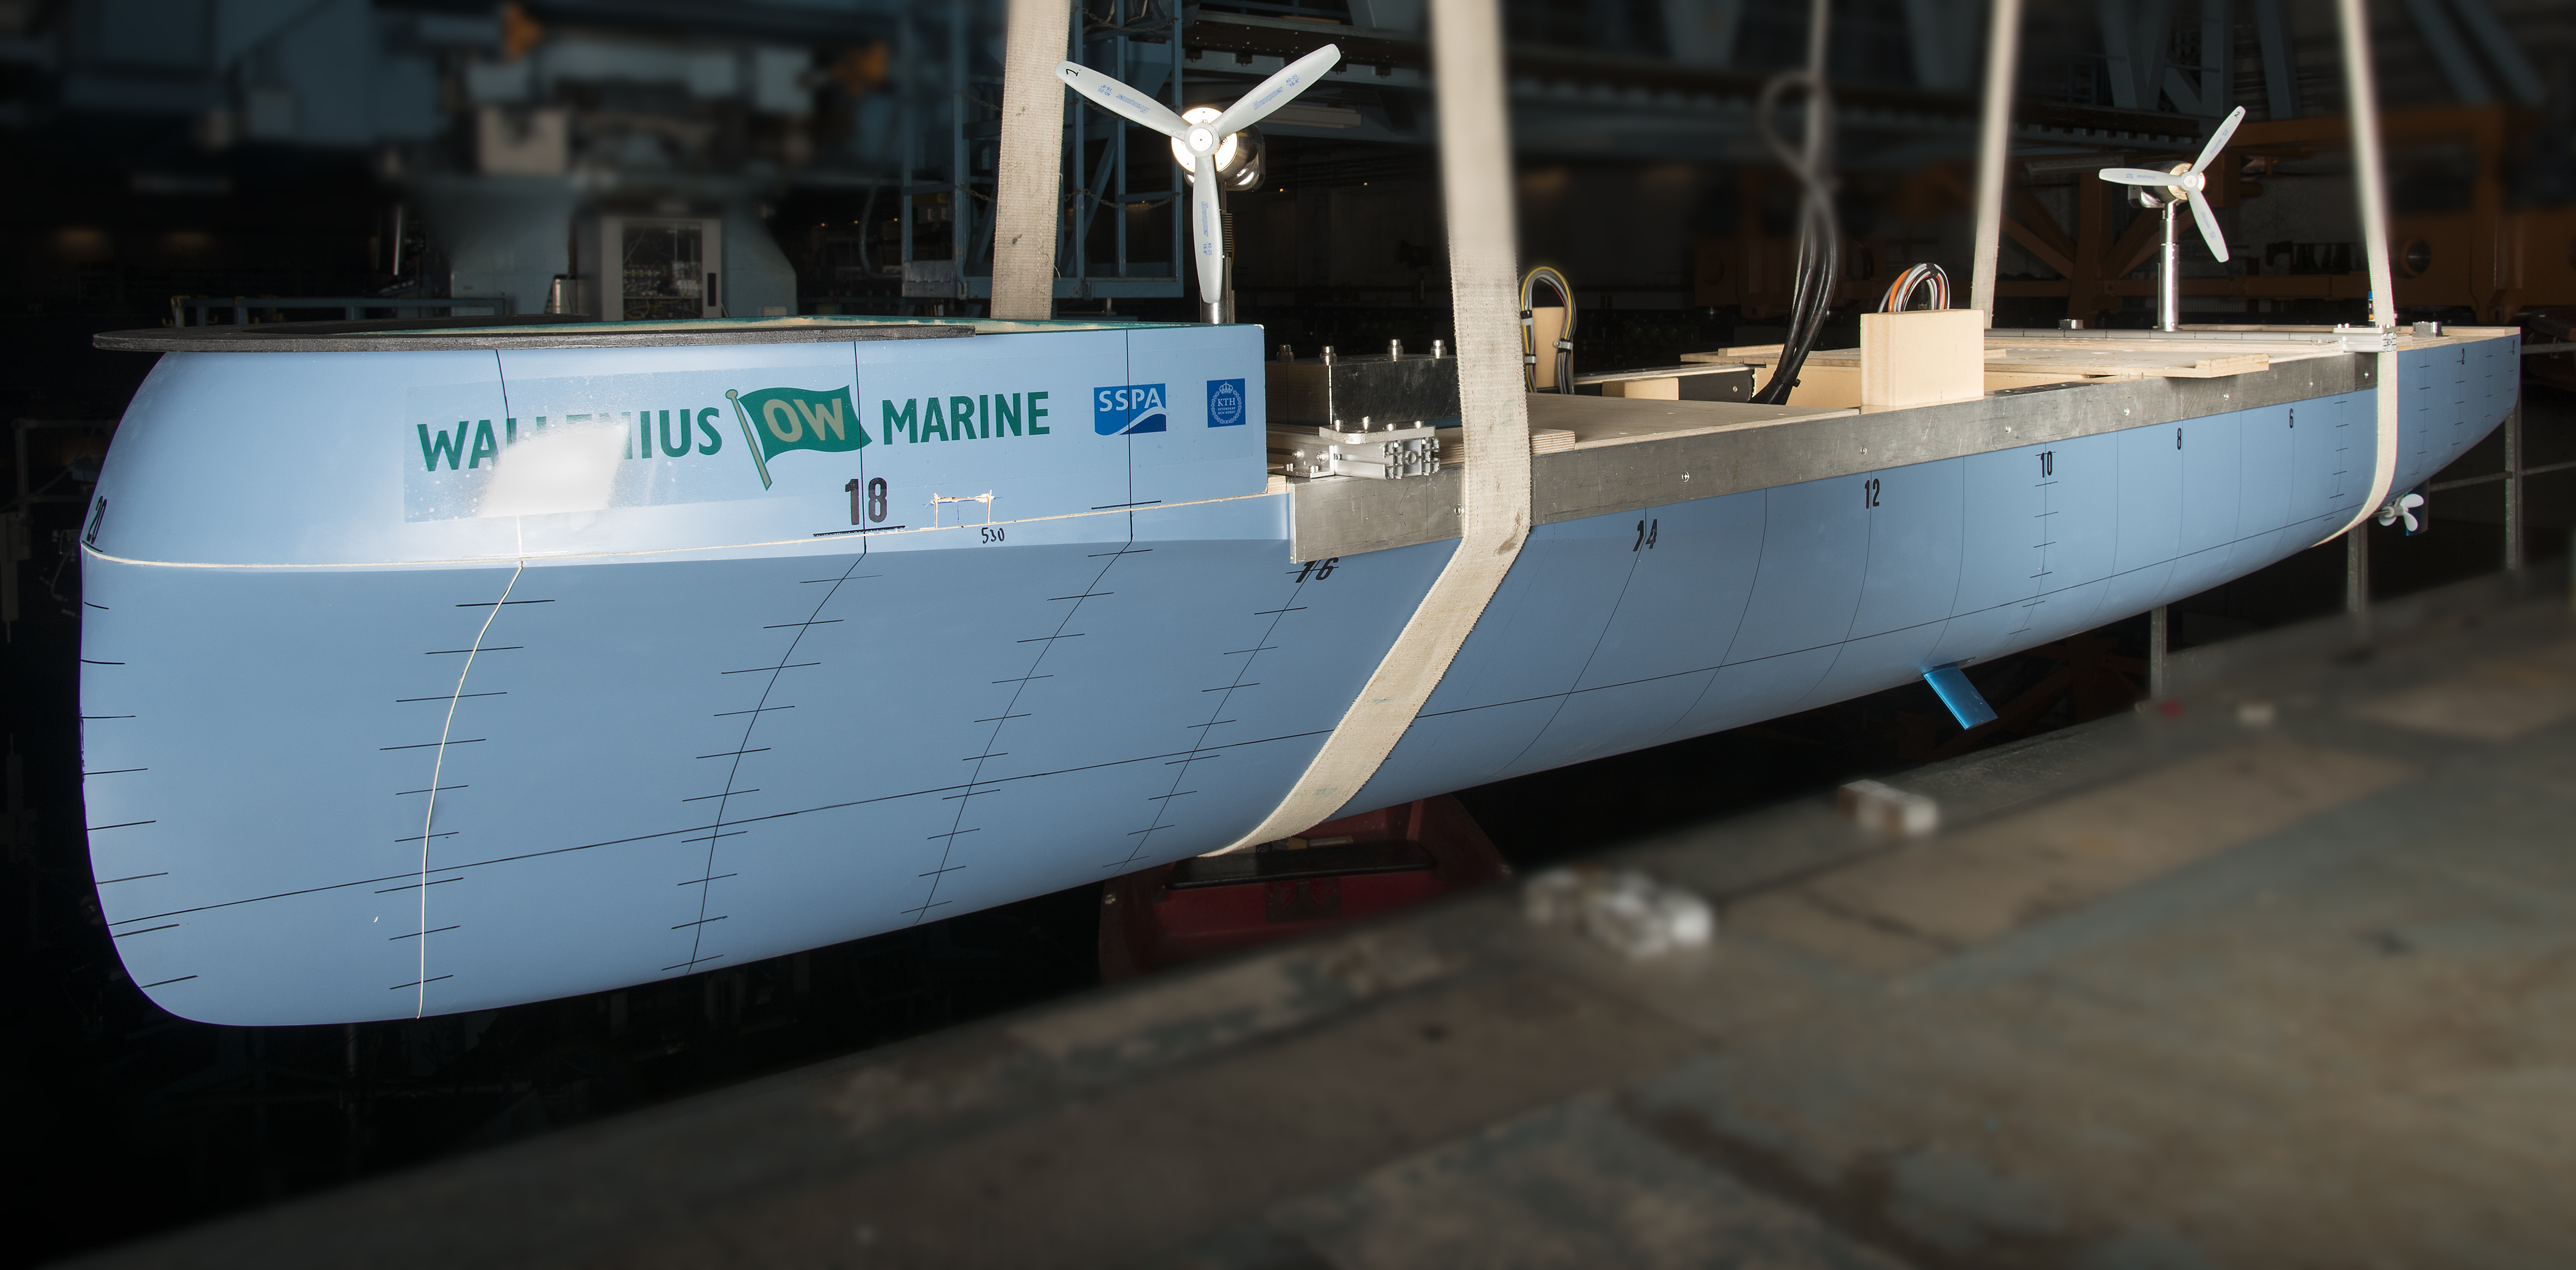
\includegraphics[width=\columnwidth]{figures/5m.jpg}
    \caption{The scale model of the WPCC used in the model tests. Copyright RISE.}
    \label{fig:WPCC}
\end{figure}